\documentclass[11pt]{article}

\usepackage[a4paper,margin=25mm]{geometry}
\usepackage[T1]{fontenc}
\usepackage{lmodern}
\usepackage{microtype}
\usepackage{amsmath,amssymb,bm}
\usepackage{graphicx}
\usepackage{booktabs}
\usepackage{array}
\usepackage{enumitem}
\usepackage{natbib}
\usepackage{placeins}
\usepackage{flafter}
\usepackage{xcolor}
\usepackage[colorlinks=true,allcolors=blue!55!black]{hyperref}

\graphicspath{{figures/}}
\setlength{\emergencystretch}{2em}
\setlist{nosep}

\newcommand{\Rey}{\mathit{Re}}
\newcommand{\dd}{\mathrm{d}}
\newcommand{\TNTI}{T/NT interface}

\title{The turbulent boundary layer as an unconfined intermittent canopy:\\
A structural synthesis}
\author{Guillem Borrell}
\date{}

\begin{document}
\maketitle

\begin{abstract}
We develop a structural interpretation of the outer region of a zero-pressure-gradient turbulent boundary layer by combining three results that are usually discussed separately: the hierarchy of wall-attached momentum-transfer and vortex structures, the time-resolved renewal of those structures, and the geometry and dynamics of the turbulent/non-turbulent interface.  The evidence supports an \emph{intermittent-canopy} picture in which self-similar motions of many sizes overlap below the boundary-layer edge, while only the largest motions reach the intermittent region.  Intense attached Reynolds-stress objects in channels have dimensions approximately proportional to their height and, at the identification threshold used in the source study, carry about 60\% of the Reynolds stress while occupying less than 8\% of a wall-parallel plane.  Related vortex clusters have comparable aspect ratios and a scale-dependent population.  Their histories are also self-similar, but they do not form literal material trees growing continuously from the wall: large objects can form away from it and repeatedly merge and split.  At the outer boundary, vorticity terminates near a threshold-dependent interface, whereas the irrotational strain outside the layer retains the potential-flow footprint of large internal motions.  Moreover, strain-normalised stretching and strain-eigenvalue statistics remain similar from the turbulent core towards the interface.  These results are consistent with the interface being the convoluted upper support of the same turbulent field that populates the logarithmic and outer layers.  They do not prove that each interface bulge is the tip of a particular attached cluster.  We therefore formulate the canopy as a constrained synthesis, distinguish direct evidence from interpretation, and propose joint object/interface measurements that would test the missing connection.
\end{abstract}

\noindent\textbf{Keywords:} wall-bounded turbulence; turbulent boundary layer; coherent structures; attached eddies; turbulent/non-turbulent interface; intermittency

\section{Introduction}

Descriptions of zero-pressure-gradient turbulent boundary layers (ZPG TBLs) commonly use several complementary languages.  Mean-flow descriptions distinguish viscous, logarithmic, wake and intermittent regions.  Structural descriptions invoke streaks, sweeps, ejections, vortex clusters and attached eddies.  Interface descriptions focus on the boundary separating rotational turbulence from the irrotational free stream \citep{CorrsinKistler1955,BorrellJimenez2016}.  These descriptions refer to different observables and cannot be identified with one another without an explicit argument.

Planar particle-image velocimetry established that the outer TBL contains repeated combinations of spanwise vorticity and strong Q2 motion \citep{AdrianEtAl2000}.  Three-dimensional direct numerical simulation (DNS) subsequently showed that intense Reynolds-stress regions and vortex clusters include wall-attached, approximately self-similar families \citep{DelAlamoEtAl2006,LozanoDuranEtAl2012}.  Time-resolved DNS added an essential qualification: geometrical attachment does not imply that an object was born at the wall or remained a single material structure throughout its life \citep{LozanoDuranJimenez2014}.  In parallel, conditional analysis of the turbulent/non-turbulent (T/NT) interface showed that the rotational and potential regions are separated by a physically meaningful vorticity boundary, while the strain induced by turbulent motions extends into the free stream \citep{BorrellJimenez2016}.

We ask whether these observations can be organised into one economical picture.  The proposed \emph{intermittent-canopy hypothesis} is:

\begin{quote}
The logarithmic and outer regions contain a hierarchy of overlapping, approximately self-similar turbulent structures. Their population and spatial coverage decrease with height. Near the boundary-layer edge, the union of the surviving structures becomes sparse, and its convoluted vortical boundary is observed as the T/NT interface.
\end{quote}

The term \emph{canopy} conveys overlap, a distribution of heights and an irregular upper envelope.  It does not imply a forest of isolated, permanent vortex tubes rooted at the wall.  The structures extracted from DNS are threshold-dependent, multiscale regions that merge and split.  In addition, most three-dimensional object evidence discussed below was obtained in channels, whereas the interface evidence was obtained in a spatially developing boundary layer.  The synthesis is plausible only to the extent that the relevant logarithmic-layer organisation is shared by the two flows.

This article is a synthesis rather than a report of a new simulation.  We consequently distinguish (i) observations displayed directly by published statistics, (ii) inferences supported by those observations, and (iii) the untested connection between the attached hierarchy and the interface.  That distinction prevents a wall-attached Reynolds-stress object, a connected vortex cluster and a region enclosed by a T/NT interface from being treated as interchangeable.

\section{Definitions and scales}

Let $x$, $y$ and $z$ denote the streamwise, wall-normal and spanwise directions.  The velocity fluctuations are $(u,v,w)$, the friction velocity is $u_\tau$, the kinematic viscosity is $\nu$, and $\delta_{99}$ is the height at which the mean velocity reaches 99\% of its free-stream value.  Wall units are denoted by a superscript $+$, so that
\begin{equation}
 \delta_{99}^{+}=\frac{u_\tau\delta_{99}}{\nu}.
\end{equation}

A quadrant object is a connected region in which the instantaneous tangential Reynolds stress exceeds a prescribed threshold.  Ejections are Q2 events ($u<0$, $v>0$), and sweeps are Q4 events ($u>0$, $v<0$).  In the object analysis of \citet{LozanoDuranEtAl2012}, an object is termed attached when its lowest point lies within approximately 20 wall units of the wall.  This is an operational definition of geometric connectivity, not a statement about the birthplace of the full object.

Let $\omega=|\bm{\omega}|$ be the vorticity magnitude.  Following \citet{BorrellJimenez2016}, a vorticity interface is constructed from an isosurface $\omega=\omega_0$, with disconnected bubbles or drops treated separately when required.  Their dimensionless interface scale is
\begin{equation}
 \omega^{*}=\omega^{+}\sqrt{\delta_{99}^{+}}
 =\omega\frac{\nu}{u_\tau^2}\sqrt{\frac{u_\tau\delta_{99}}{\nu}}.
 \label{eq:star}
\end{equation}
The corresponding dimensional edge-vorticity scale is
\begin{equation}
 \omega_e\sim \frac{u_\tau^2}{\nu\sqrt{\delta_{99}^{+}}}
 =\sqrt{\frac{u_\tau^3}{\nu\delta_{99}}},
\end{equation}
up to constants.  It follows from the local-equilibrium estimate $\nu\omega_e^2\sim u_\tau^3/\delta_{99}$.  Note that $\sqrt{\delta_{99}^{+}}$, rather than its inverse, appears in the definition of $\omega^*$.

For a chosen threshold, the turbulent fraction is
\begin{equation}
 \gamma(y;\omega_0)=\Pr\{\omega(x,y,z)>\omega_0\}.
 \label{eq:gamma}
\end{equation}
If the interface were a single-valued height $y_I(x,z)$, without overhangs or pockets, equation~\eqref{eq:gamma} would reduce approximately to
\begin{equation}
 \gamma(y;\omega_0)\simeq \Pr\{y_I(x,z;\omega_0)>y\}.
\end{equation}
It is not generally equal to $\Pr\{h_k>y\}$, where $h_k$ is a cluster height.  Pointwise coverage also depends on each object's footprint, overlap, threshold and connectivity.  A cluster-height cumulative distribution is therefore not, by itself, an intermittency profile.

\section{A self-similar structural hierarchy}
\label{sec:hierarchy}

\subsection{Three-dimensional attached objects}

The vortex-cluster analysis of \citet{DelAlamoEtAl2006} separates compact detached objects from tall attached objects.  Rather than using one arbitrarily selected cluster as evidence for the hierarchy, figure~\ref{fig:vortex-scaling} shows the population statistics directly.  The Cartesian bounding dimensions scale approximately as
\begin{equation}
 \Delta_x\simeq 3\Delta_y,\qquad \Delta_z\simeq 1.5\Delta_y.
 \label{eq:vortex-aspect}
\end{equation}
The data in figure~\ref{fig:vortex-scaling} are from the S1900 channel at $\Rey_\tau\simeq1900$, comparable to the upper friction-Reynolds-number range of the boundary-layer interface data discussed in section~\ref{sec:interface}.  Reynolds number is therefore not the main mismatch between the two datasets; flow geometry and object definition are.  Figure~\ref{fig:vortex-scaling} establishes a channel hierarchy but does not identify a channel cluster with a boundary-layer interface patch.

The number density per unit wall area and height has a power-law tail.  As the identification threshold approaches the percolation transition, its exponent approaches $-3$, as expected for a Townsend-like geometrically self-similar population \citep{Townsend1976,DelAlamoEtAl2006}.

\begin{figure}[tb]
 \centering
 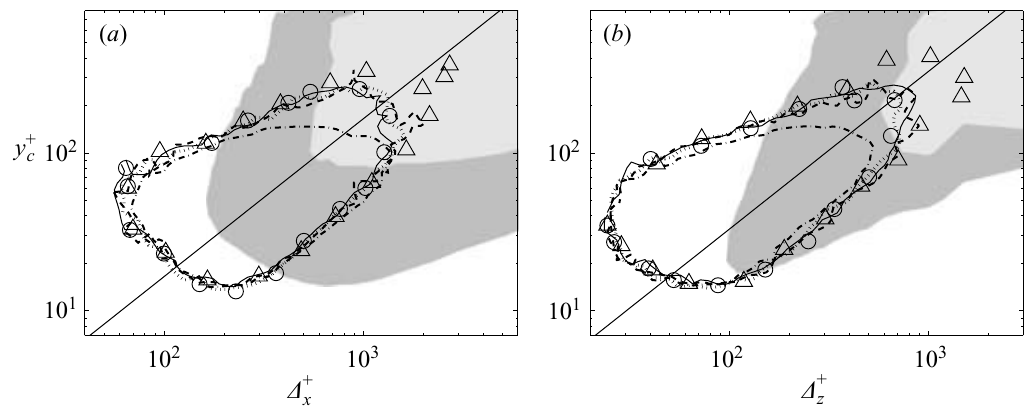
\includegraphics[width=0.88\linewidth]{vortex-cluster-scaling.png}
 \caption{Joint distributions of attached-cluster streamwise (a) and spanwise (b) dimensions versus the wall distance of their centres. The diagonal trends are the direct evidence for geometrical self-similarity. Data are from the S1900 channel at $\Rey_\tau\simeq1900$. Reproduced from figure~7 of \citet{DelAlamoEtAl2006}.}
 \label{fig:vortex-scaling}
\end{figure}

\citet{LozanoDuranEtAl2012} performed a corresponding three-dimensional analysis of intense momentum-transfer events.  Their objects separate into attached and detached populations (figure~\ref{fig:q-stress}).  At their selected threshold, attached Q2 and Q4 objects occupy less than 8\% of a wall-parallel plane but account for approximately 60\% of the mean Reynolds shear stress at all heights.  This threshold-specific statement is more defensible than claiming that such objects fill the flow or carry nearly all of the stress.

\begin{figure}[tb]
 \centering
 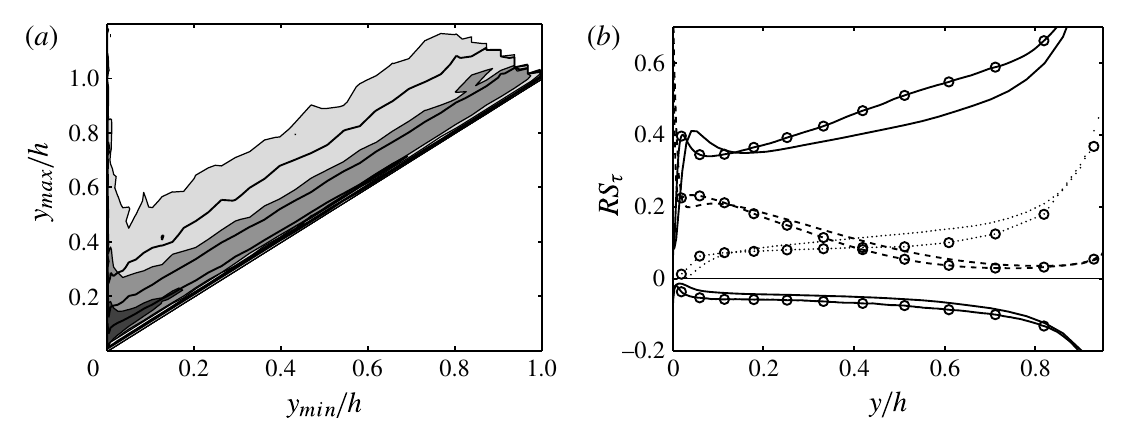
\includegraphics[width=0.92\linewidth]{q-stress.png}
 \caption{Left: joint distribution of the lowest and highest wall distances of identified Q objects. Right: fractional contributions to Reynolds stress from attached Q2 and Q4 objects, detached objects and counter-gradient events. Reproduced from figure~2 of \citet{LozanoDuranEtAl2012}.}
 \label{fig:q-stress}
\end{figure}

The attached Q family has dimensions
\begin{equation}
 \Delta_x\simeq 3\Delta_y,\qquad \Delta_z\simeq \Delta_y,
 \label{eq:q-aspect}
\end{equation}
except for the largest objects crossing the channel centreline.  Figure~\ref{fig:q-sizes} displays the distributions underlying equation~\eqref{eq:q-aspect}.  The similarity between equations~\eqref{eq:vortex-aspect} and \eqref{eq:q-aspect} is significant, but it does not imply that the vortex and momentum-transfer objects are identical.  More than 80\% of attached vortex clusters intersect a Q object, whereas the reverse probability decreases with height because tall Q objects outnumber tall clusters \citep{LozanoDuranEtAl2012}.

\begin{figure}[tb]
 \centering
 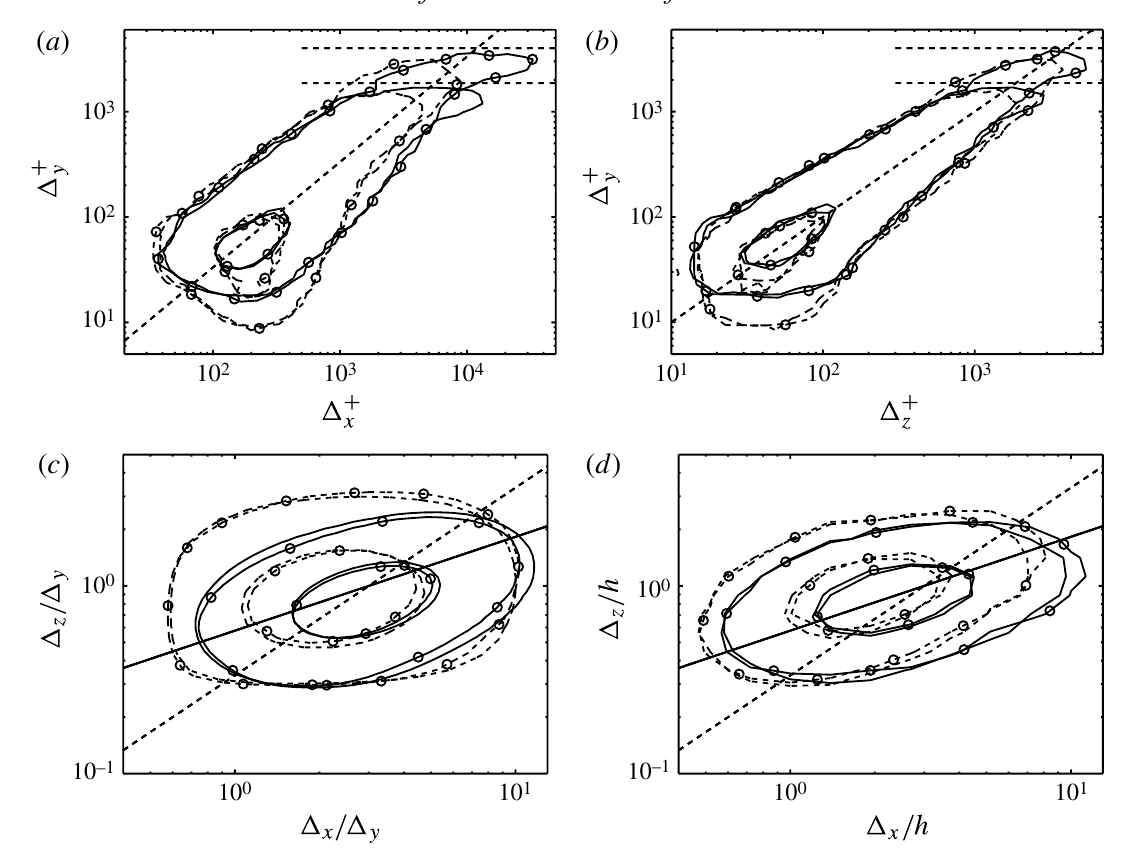
\includegraphics[width=0.82\linewidth]{q-sizes.png}
 \caption{Joint distributions of the dimensions of attached Q2 and Q4 objects.  The diagonal trends in panels (a,b) support dimensions proportional to object height.  The largest objects in panel (d) depart from the simpler self-similar family. Reproduced from figure~5 of \citet{LozanoDuranEtAl2012}.}
 \label{fig:q-sizes}
\end{figure}

The preferred arrangement is a side-by-side Q2--Q4 pair with a vortex cluster associated with the Q2 and with the shear layer below the Q4.  Figure~\ref{fig:q-pair} compares the conditional geometry with one instantaneous realisation.  The instantaneous field is appreciably less regular than its conditional average.

\begin{figure}[tb]
 \centering
 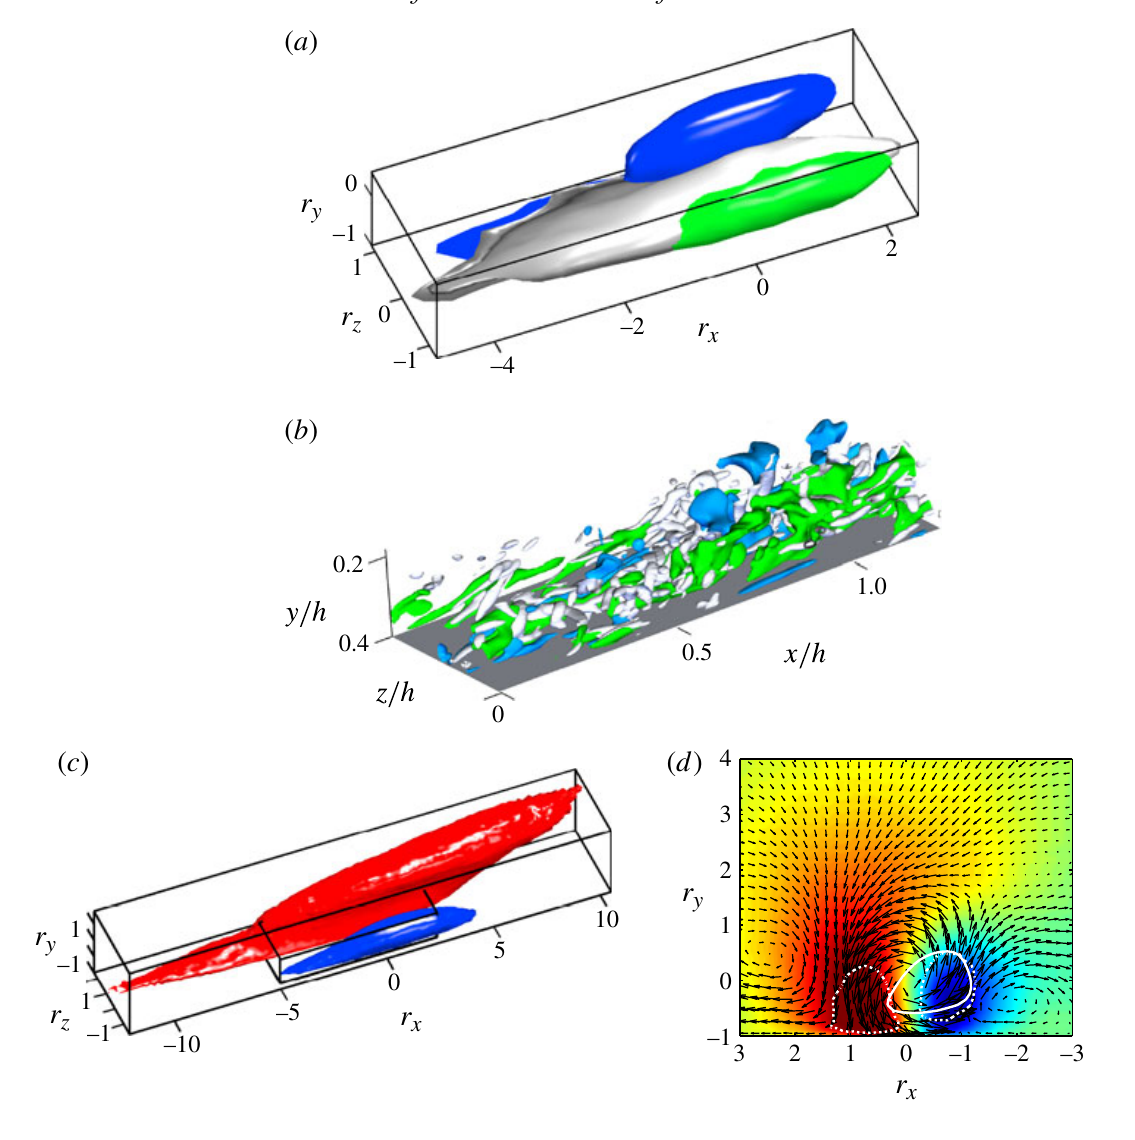
\includegraphics[width=0.73\linewidth]{q-pair.png}
 \caption{Conditional geometry, an instantaneous realisation, and the associated velocity field of a Q2--Q4 pair. Green denotes Q2, blue Q4 and grey the vortex cluster in the upper panels. Reproduced from figure~12 of \citet{LozanoDuranEtAl2012}.}
 \label{fig:q-pair}
\end{figure}

These observations provide three ingredients of the canopy interpretation: objects span a hierarchy of heights; their wall-parallel dimensions grow with height; and sparse intense objects make a disproportionate contribution to momentum transfer.  They do not make velocity, stress and vorticity thresholds interchangeable.

\subsection{The largest objects are composite}

Self-similarity breaks down for the largest channel structures.  Objects crossing the centreline account for roughly one third of the stress carried by attached Q objects. Fewer than 1\% of all identified objects account for about 60\% of the volume of the attached population, and streamwise lengths can approach $20\delta$ \citep{LozanoDuranEtAl2012}. Figure~\ref{fig:q-composite} shows that a very-large Q2 is visibly assembled from smaller pieces.

\begin{figure}[tb]
 \centering
 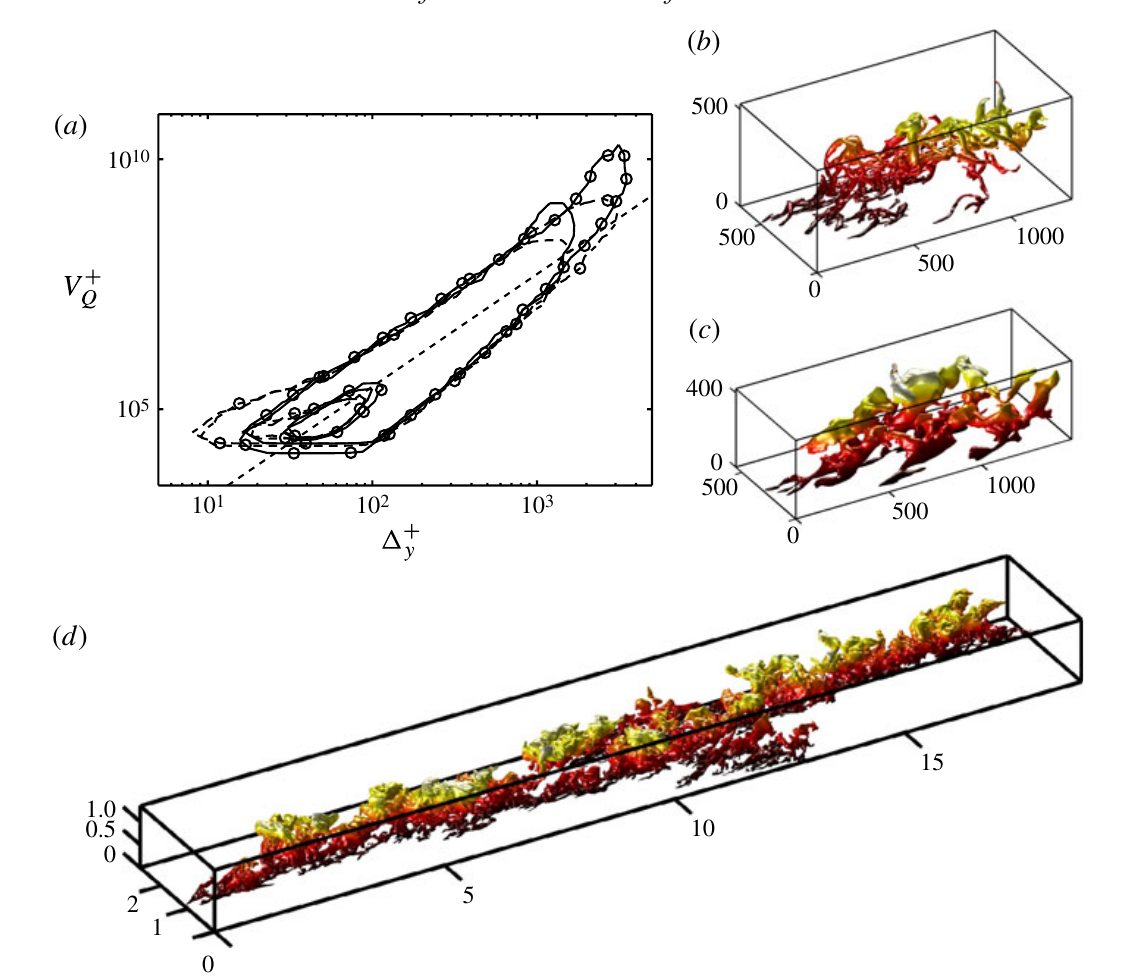
\includegraphics[width=0.80\linewidth]{q-composite.png}
 \caption{An attached vortex cluster (b), an attached Q2 (c) and a very-large centreline-crossing Q2 (d).  The global object is visibly composite. Reproduced from figure~8 of \citet{LozanoDuranEtAl2012}.}
 \label{fig:q-composite}
\end{figure}

Consequently, the height of a percolated object is not necessarily the size of one dynamical eddy, and a long correlation or spectral mode need not represent one continuous vortex packet.  Spectral evidence likewise contains multiple geometrical regimes: the width of the streamwise-velocity spectrum varies approximately as the square root of its length, and the largest global modes require an outer velocity scale \citep{DelAlamoEtAl2004}.  Any canopy model must distinguish active momentum-transfer motions from longer, partly inactive streamwise-velocity organisation.

\subsection{Time evolution: a renewing canopy}

Time-resolved tracking changes the meaning of attachment. \citet{LozanoDuranJimenez2014} found geometrically self-similar tall branches whose lifetimes scale approximately as
\begin{equation}
 \frac{Tu_\tau}{\Delta_y}=O(1).
 \label{eq:lifetime}
\end{equation}
Detached objects instead have sizes and lifetimes controlled by local dissipative scales (figure~\ref{fig:lifetimes}).

\begin{figure}[tb]
 \centering
 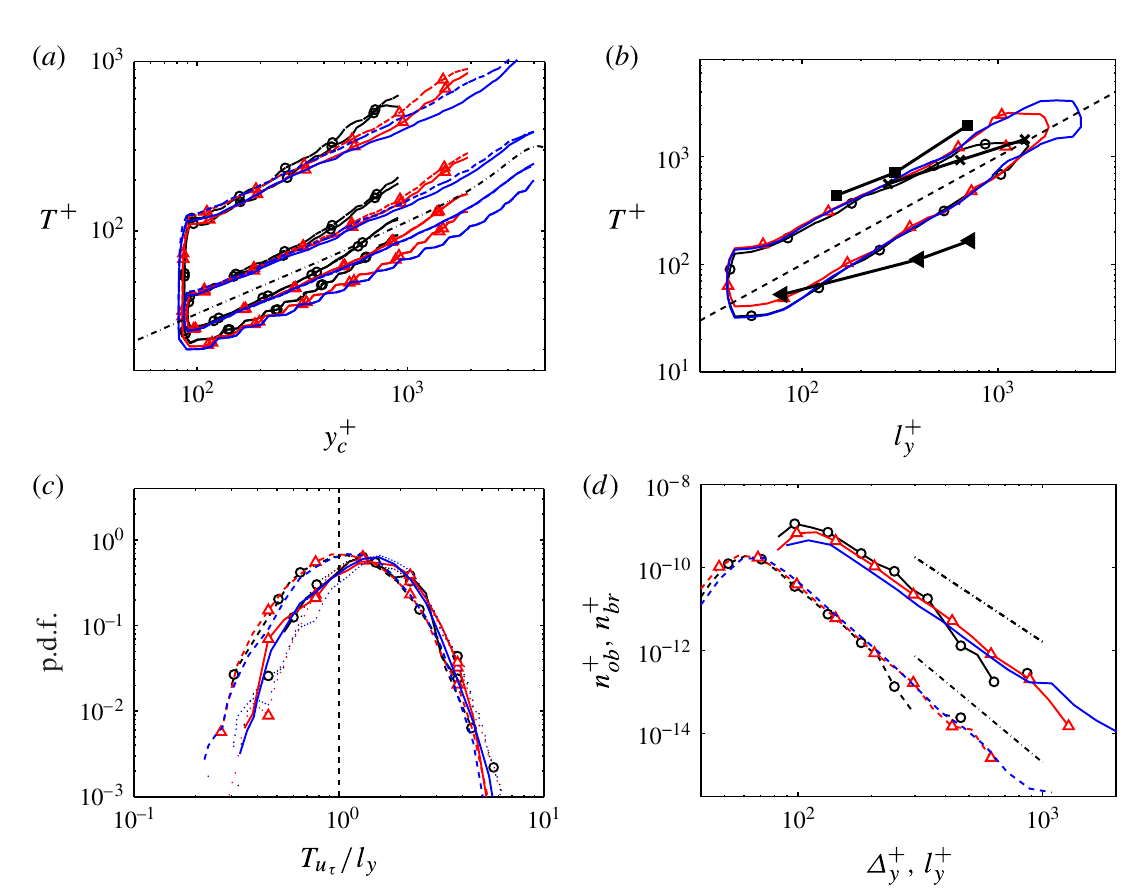
\includegraphics[width=0.82\linewidth]{lifetimes.png}
 \caption{Lifetime statistics of detached and tall attached coherent structures. Panel (a) follows a local dissipative time, whereas panels (b,c) show the height-scaled lifetime of tall attached objects. Reproduced from figure~9 of \citet{LozanoDuranJimenez2014}.}
 \label{fig:lifetimes}
\end{figure}

Figure~\ref{fig:birth-death} reveals an approximate sweep--ejection symmetry.  Ejections tend to appear near the wall and move away from it; sweeps tend to appear aloft and move towards it; vortex clusters broadly follow the ejections.  Thus, ``attached'' does not imply that every large object begins as a small wall object and is convected intact to the edge.  Indeed, the vertical speed required for all tall clusters to grow continuously from the wall would be unrealistically large \citep{DelAlamoEtAl2006}.

\begin{figure}[tb]
 \centering
 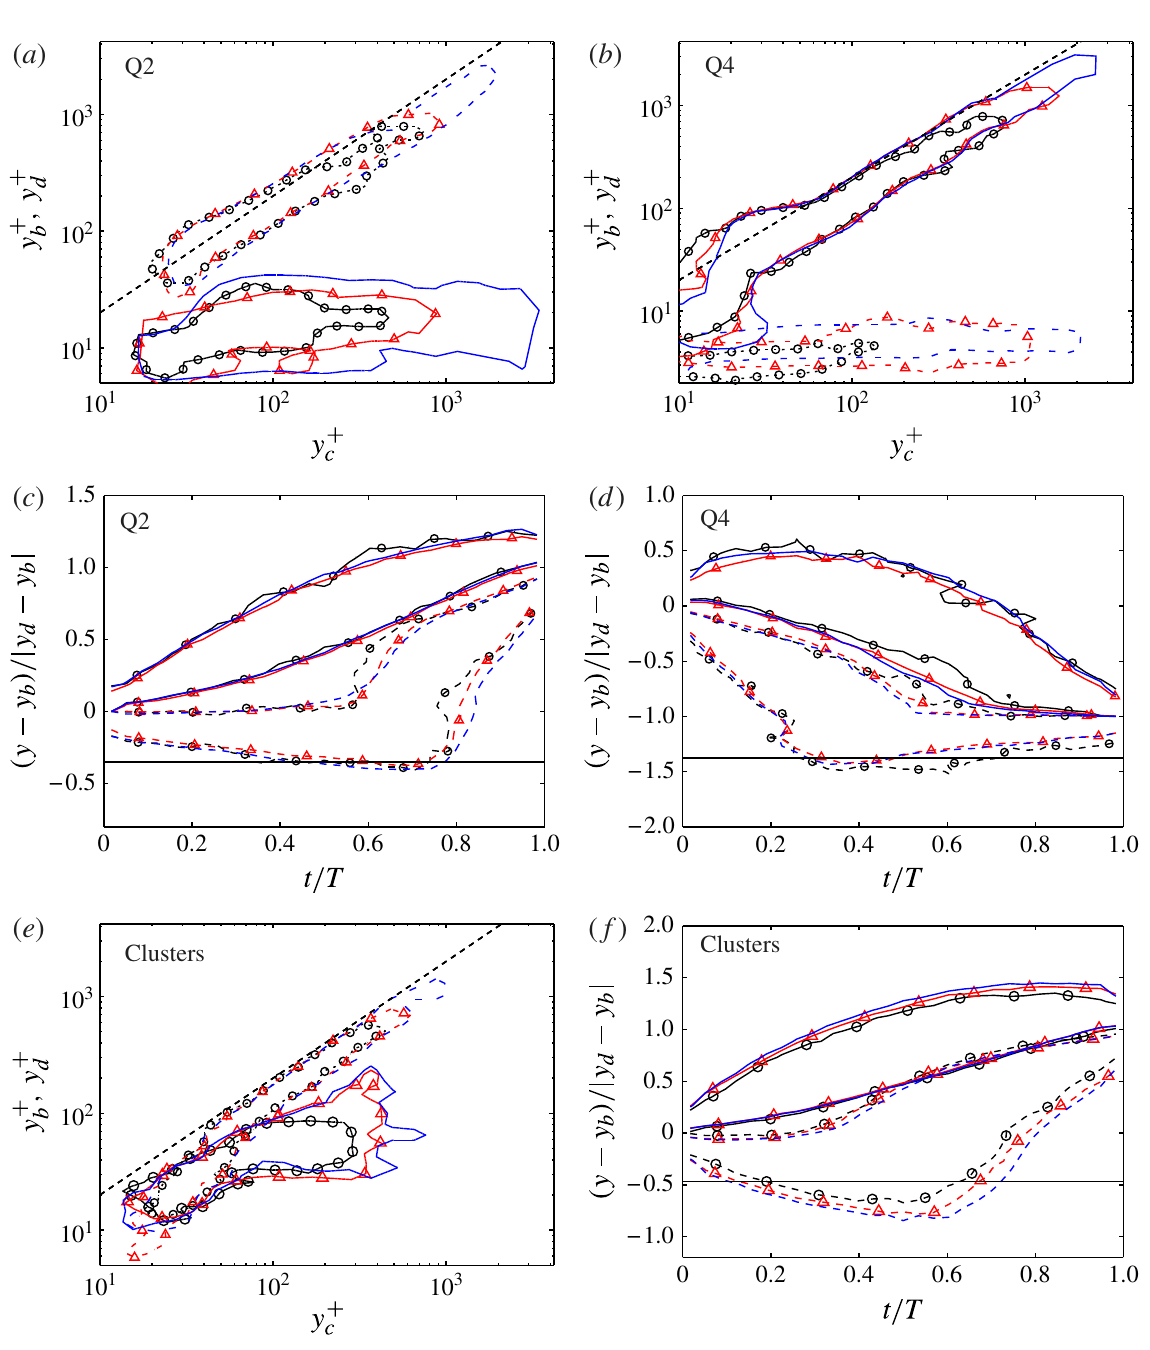
\includegraphics[width=0.73\linewidth]{birth-death.png}
 \caption{Birth/death positions and vertical histories of ejections (a,c), sweeps (b,d) and vortex clusters (e,f).  The contrast between Q2 and Q4 histories argues against a universal bottom-up trajectory. Reproduced from figure~11 of \citet{LozanoDuranJimenez2014}.}
 \label{fig:birth-death}
\end{figure}

Merging and splitting are also integral to object histories.  Structures smaller than approximately $30\eta$ rarely participate, while almost all structures larger than approximately $100\eta$ do.  Mergers occur preferentially early in a branch lifetime and splits late (figure~\ref{fig:merger-split}).  The direct direction dominates, but inverse events are not negligible.

\begin{figure}[tb]
 \centering
 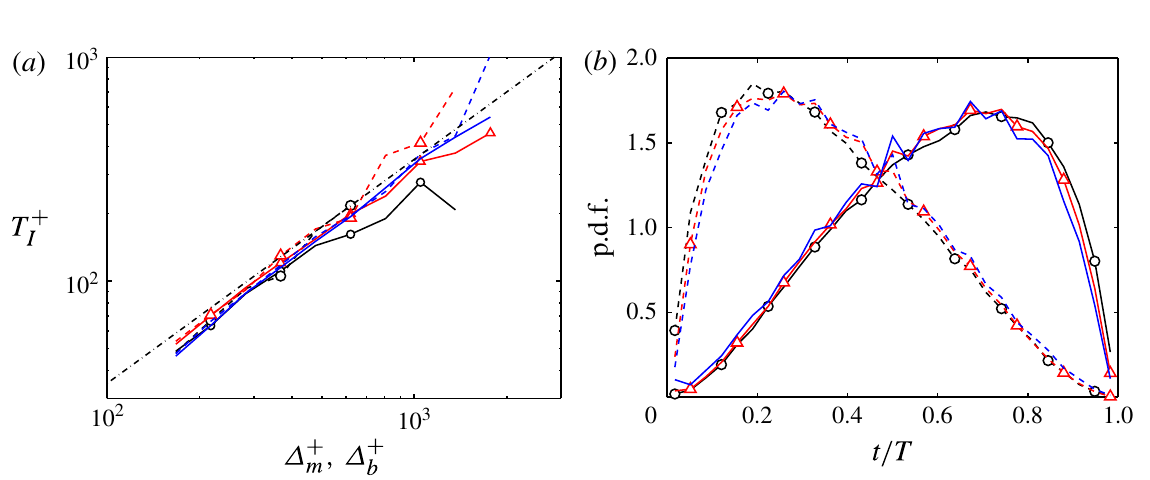
\includegraphics[width=0.84\linewidth]{merger-split.png}
 \caption{Similar-size interaction time versus fragment size (a) and the time of mergers (dashed) and splits (solid) within a branch lifetime (b). Reproduced from figure~20 of \citet{LozanoDuranJimenez2014}.}
 \label{fig:merger-split}
\end{figure}

The tracked quantity in this analysis is the volume of an intense Reynolds-stress or vortex object, not spectral kinetic-energy flux.  The resulting geometrical cascade need not coincide with the Kolmogorov energy cascade \citep{LozanoDuranJimenez2014}.  The appropriate picture is therefore a \emph{renewing canopy}, not a set of persistent material branches.

\FloatBarrier
\section{The intermittent edge}
\label{sec:interface}

\subsection{A threshold-dependent vorticity boundary}

Velocity and strain fluctuations can exist in irrotational fluid.  Pressure and potential velocity induced by turbulence below the edge extend outside the vortical region, so velocity- or energy-based thresholds need not identify rotational turbulence.  \citet{BorrellJimenez2016} show that vorticity isosurfaces have a sharper physical status than strain isosurfaces: both vorticity and strain change sharply when distance is measured from a vorticity interface, but an equivalent transition is absent when distance is measured from a strain interface.

The vorticity boundary is nevertheless threshold dependent.  Figure~\ref{fig:threshold} renders the same DNS region at thresholds differing by one decade.  The lower threshold behaves as a relatively smooth outer envelope, whereas the higher threshold penetrates the core and develops handles and deep convolutions.  The fractal dimension and genus undergo a transition as the threshold moves from the free stream into the turbulent core \citep{BorrellJimenez2016}.  Any canopy statement must therefore report its threshold.

\begin{figure}[tb]
 \centering
 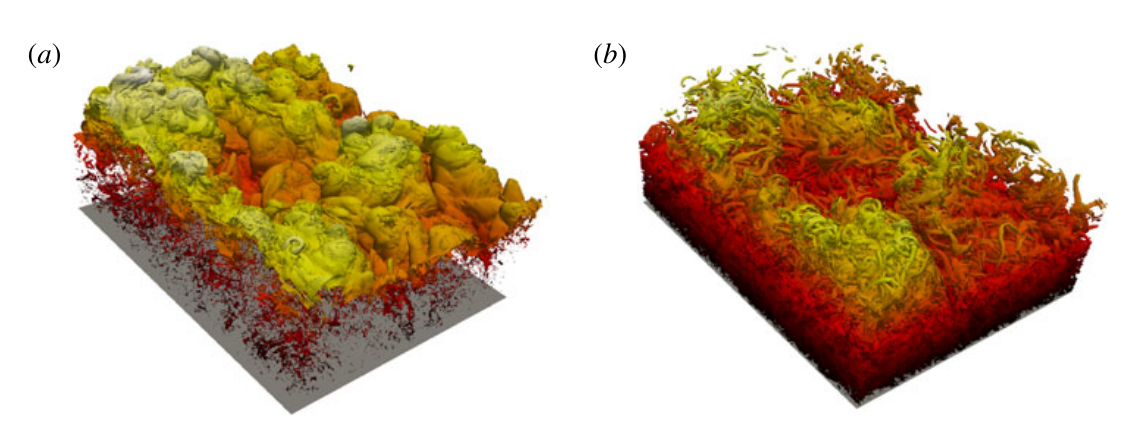
\includegraphics[width=0.92\linewidth]{interface-threshold.png}
 \caption{Vorticity isosurfaces of the same boundary-layer region at thresholds differing by one decade. The low-threshold surface (a) behaves as an outer envelope, whereas the higher-threshold surface (b) penetrates the turbulent field and is more multiply connected. Reproduced from figure~2 of \citet{BorrellJimenez2016}.}
 \label{fig:threshold}
\end{figure}

Overhangs and pockets prevent the interface from being represented exactly by a single-valued canopy height.  Their existence is relevant to equation~\eqref{eq:gamma}; their detailed size distribution and viscous diffusion thickness do not, by themselves, test whether attached clusters form the canopy.  Those interface properties are therefore not used as supporting links in the present argument.

\subsection{The exterior strain as the shadow of internal motions}

Figure~\ref{fig:outer-strain} is a direct bridge from the turbulent field to the irrotational exterior.  Vorticity falls rapidly above the boundary-layer edge, but strain persists into the free stream.  Its decay follows the potential-flow behaviour associated with wall-parallel wavelengths of order $2\delta_{99}$.  The exterior strain is therefore not evidence for a second vortical population.  It can be interpreted as the irrotational footprint, or ``shadow'', of the largest internal motions.

\begin{figure}[tb]
 \centering
 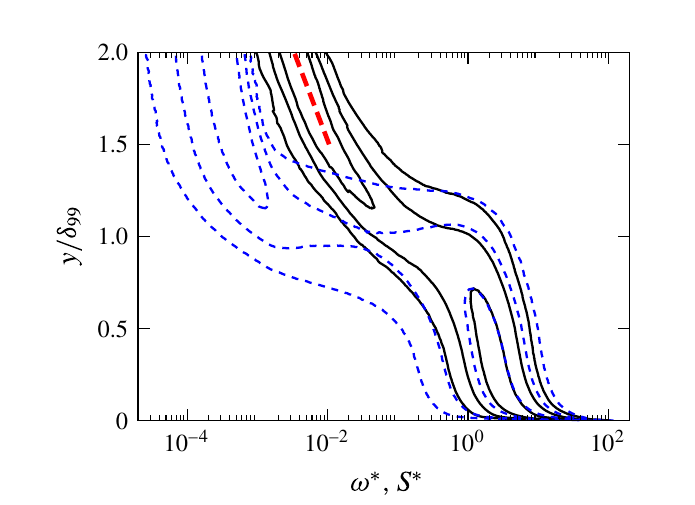
\includegraphics[width=0.62\linewidth]{outer-strain.png}
 \caption{Joint wall-normal distributions of vorticity (blue dashed contours) and strain (black solid contours). Vorticity terminates rapidly, while strain extends into the free stream along the potential-flow decay marked in red. Reproduced from figure~20 of \citet{BorrellJimenez2016}.}
 \label{fig:outer-strain}
\end{figure}

This result supplies a precise interpretation of the canopy metaphor.  The vortical canopy has a finite, intermittent support, but the velocity and pressure fields induced by it do not terminate on that support.  An observer using velocity or strain alone can therefore detect the canopy above the vorticity interface without detecting rotational turbulence there.

\subsection{Core-to-interface continuity}

Figure~\ref{fig:interface-straining} provides the strongest evidence that the interface does not introduce a qualitatively separate local straining mechanism.  Panel (a) follows the joint vorticity and strain distributions towards the interface, and panel (b) follows vortex stretching and compression.  In panels (c,d), stretching/compression and strain eigenvalues are normalised by local strain. Their distributions at $7\eta$ and $100\eta$ from the interface are similar.

\begin{figure}[tb]
 \centering
 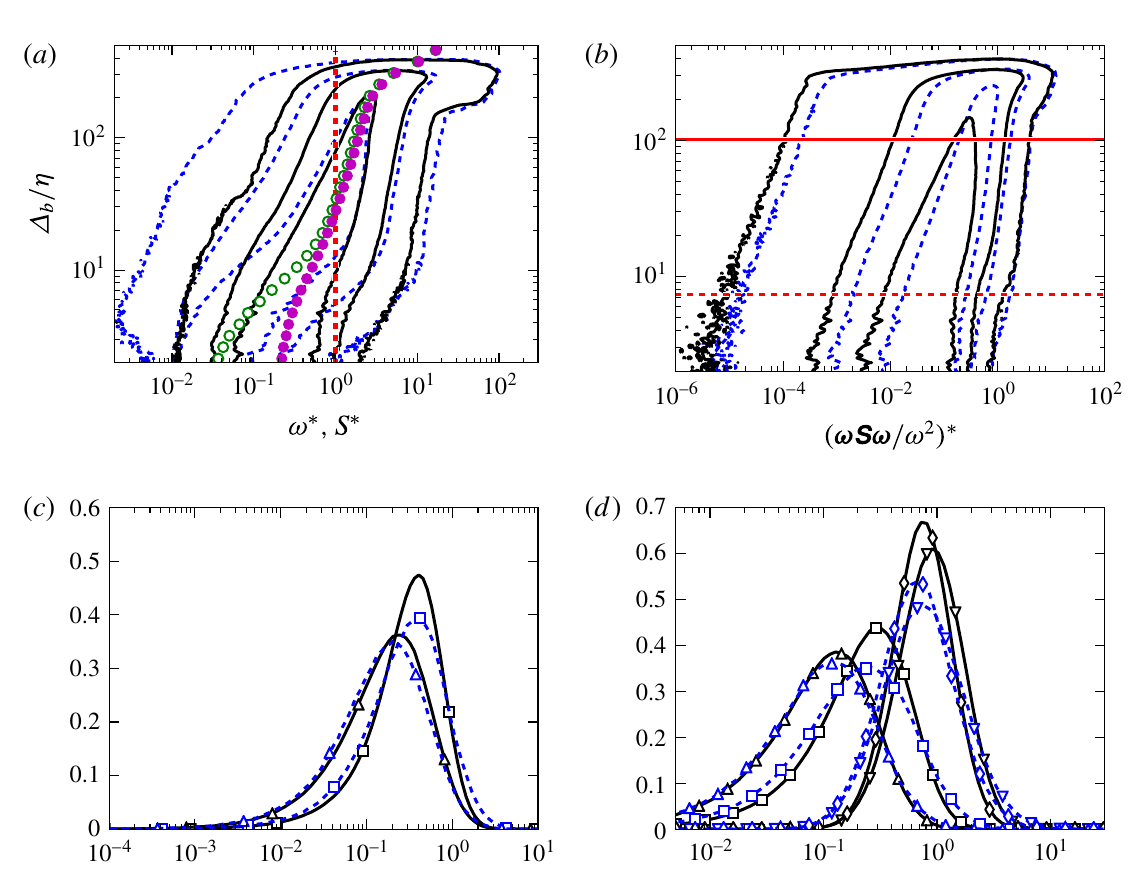
\includegraphics[width=0.84\linewidth]{interface-straining.png}
 \caption{Conditional gradient statistics relative to the vorticity interface. Blue dashed curves in panels (c,d) are sampled at $7\eta$ and black solid curves at $100\eta$. Their near collapse after local-strain normalisation shows that the interface retains the straining organisation of the core. Reproduced from figure~23 of \citet{BorrellJimenez2016}.}
 \label{fig:interface-straining}
\end{figure}

The vorticity amplitude is extinguished across the edge without a corresponding replacement of the local strain geometry.  This supports continuity between the turbulent core and its upper boundary more directly than interface geometry alone.  It still does not identify which Q object or vortex cluster supplies a particular interface patch, because the conditional average contains no cluster labels.

The same source also measures a Taylor-microscale interface thickness and a thinner viscous diffusion range.  Those are important for interface physics and numerical resolution, but no relation is established between either thickness and the height, spacing, population or lifetime of the attached structures.  The particular T/NT-interface thickness is consequently peripheral to the canopy framework.

\FloatBarrier
\section{The canopy synthesis and its limits}
\label{sec:synthesis}

The object and interface datasets fit together at four levels:
\begin{enumerate}
 \item attached vortex and momentum-transfer families supply structures over a broad range of heights;
 \item their dimensions grow and their population decreases with size;
 \item the largest attached motions influence the full layer and the near-wall region;
 \item the rotational support ends at a convoluted vorticity boundary, while the potential strain footprint and the locally normalised straining organisation remain continuous with the internal turbulence.
\end{enumerate}
This combination motivates interpreting the intermittent region as the sparse upper support of a hierarchy rather than as a separate sheet placed above an otherwise complete outer flow.  It also explains why a planar section can suggest isolated bulges or packets even when the three-dimensional field is strongly connected.

The decisive one-to-one test has not yet been performed in the cited work.  Establishing that a T/NT-interface bulge is the tip of a particular attached object requires vorticity clusters, Q structures and the interface to be extracted simultaneously from the same TBL snapshots.  The observation that more than 80\% of channel vortex clusters intersect a Q object is encouraging, but it is neither a boundary-layer result nor an interface result.

A similarly careful statement is required for vorticity.  For incompressible, constant-density flow,
\begin{equation}
 \frac{D\bm{\omega}}{Dt}
 = (\bm{\omega}\!\cdot\!\nabla)\bm{u}+\nu\nabla^2\bm{\omega}.
 \label{eq:vorticity}
\end{equation}
There is no baroclinic source in equation~\eqref{eq:vorticity}.  The wall supplies vorticity, stretching and tilting redistribute and amplify it, and viscosity diffuses it across the T/NT interface.  This global statement does not imply a Lagrangian conveyor belt in which identifiable vortex objects travel intact from the wall to $\delta_{99}$.  The tracking evidence argues against that literal interpretation.

\section{Boundary layers and channels}
\label{sec:comparison}

A channel is not a boundary layer with a reflecting outer boundary.  \citet{JimenezEtAl2010} show that large-scale velocity correlations cross the channel centreline; ejections from one half can penetrate the other.  A TBL replaces this centreline interaction with an intermittent mixture of rotational and potential fluid and with associated pressure fluctuations.  Figure~\ref{fig:centreline} demonstrates centreline coupling but does not demonstrate a destructive collision between two attached hierarchies.

\begin{figure}[tb]
 \centering
 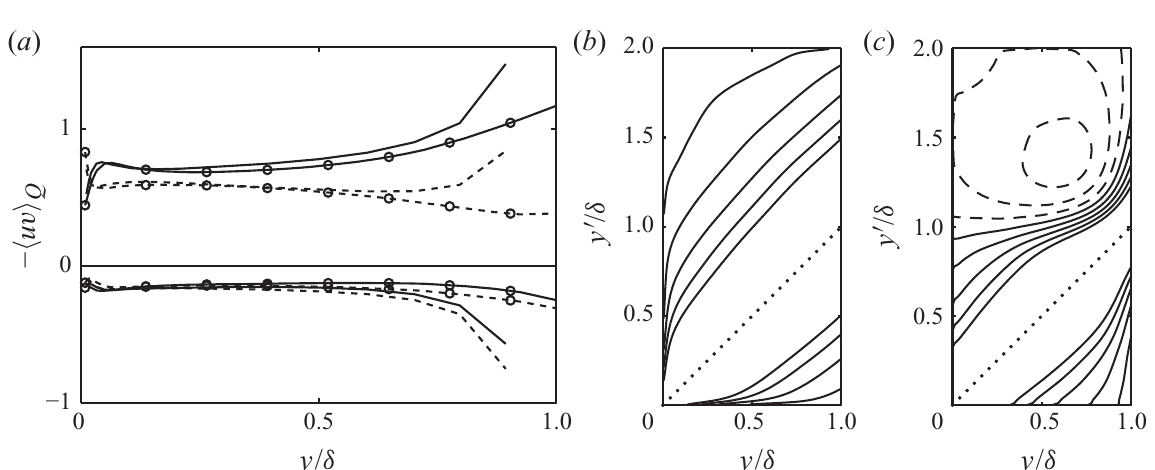
\includegraphics[width=0.93\linewidth]{centreline-coupling.png}
 \caption{Quadrant contributions in a channel and a boundary layer (a), and wall-normal (b) and streamwise (c) large-scale channel correlations. Contours crossing $y/\delta=1$ demonstrate centreline coupling. Reproduced from figure~5 of \citet{JimenezEtAl2010}.}
 \label{fig:centreline}
\end{figure}

Higher-Reynolds-number one-point statistics show that all three velocity-component intensities exceed their channel values in the TBL, with the largest difference near $y/\delta\simeq0.35$--$0.5$ and little movement of that location over the available Reynolds-number range \citep{SilleroEtAl2013}.  This is consistent with an edge-mediated pressure and entrainment effect, not with a dynamically empty outer TBL.

Three-dimensional correlations provide the strongest correction to the earlier ``channel traffic jam'' interpretation \citep{SilleroEtAl2014}.  Weak streamwise-velocity correlations reach approximately $18\delta$ in channels but only approximately $7\delta$ in boundary layers.  Their cross-flow organisation is nevertheless qualitatively similar.  Figure~\ref{fig:corr-lengths} shows that the channel streamwise correlation length continues to grow to $y/\delta\simeq0.5$, while the boundary-layer value levels off much earlier.  The source study argues that intermittency prevents the corresponding global structure from forming in the TBL.

\begin{figure}[tb]
 \centering
 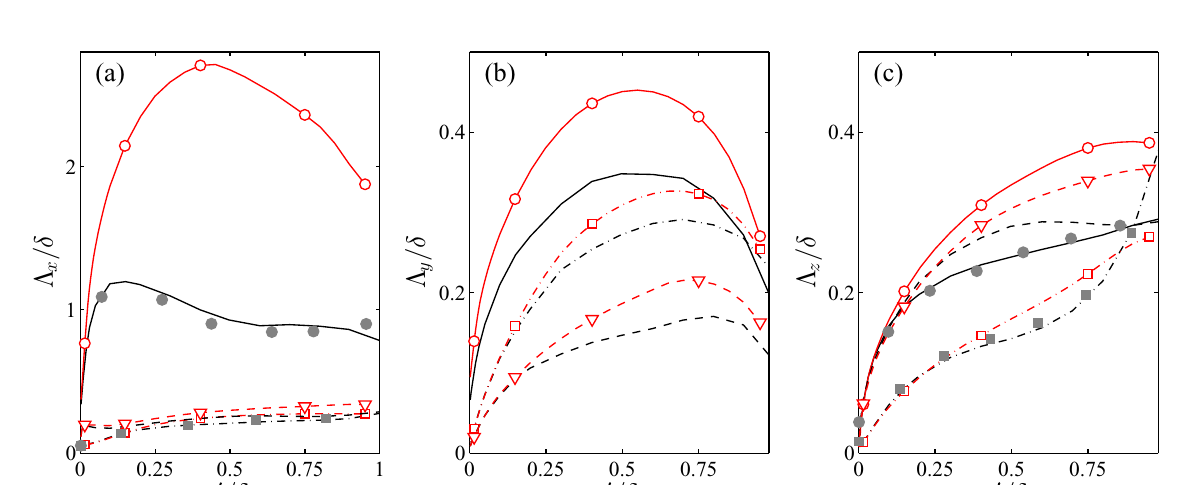
\includegraphics[width=0.92\linewidth]{correlation-lengths.png}
 \caption{Integral correlation lengths for the three velocity components. In panel (a), the red channel curve for streamwise velocity continues to grow to $y/\delta\simeq0.5$, whereas the black boundary-layer curve levels off earlier. Reproduced from figure~10 of \citet{SilleroEtAl2014}.}
 \label{fig:corr-lengths}
\end{figure}

The defensible comparison is therefore:
\begin{itemize}
 \item a channel has no T/NT interface, communicates across its centreline and supports very long global streamwise modes;
 \item a boundary layer has an open intermittent edge, stronger pressure and transverse-velocity fluctuations, shorter streamwise correlations and a potential-flow footprint beyond the vorticity boundary.
\end{itemize}
``Unconfined'' does not mean dynamically simpler.  It means that the outer boundary condition is an irrotational free stream rather than another turbulent half-channel.

\FloatBarrier
\section{Direct tests of the hypothesis}

The canopy interpretation can be tested quantitatively using existing DNS fields or modest extensions of them.

\subsection{Joint object/interface labelling}
For each snapshot and several $\omega_0^*$, identify the cleaned T/NT interface, attached vortex clusters and attached Q objects.  Measure
\begin{equation}
 P\!\left(d_{\mathrm{TNTI}}<a\lambda\mid\text{top of attached object}\right)
\end{equation}
and compare it with randomised objects of the same size and height.  A canopy interpretation predicts an excess near the tops of the largest objects, robust over the low-threshold side of the topological transition.

\subsection{Coverage rather than height alone}
Construct the pointwise union of objects and compare its coverage
\begin{equation}
 \gamma_Q(y;H)=\Pr\{(x,y,z)\in\cup_k Q_k(H)\}
\end{equation}
with the vorticity intermittency in equation~\eqref{eq:gamma}.  Object footprints and overlaps must be retained; a cumulative height distribution is insufficient.

\subsection{Conditional budgets at structural tips}
Evaluate mean-shear production, nonlinear transport, vortex stretching and viscous diffusion conditioned jointly on distance from the interface and distance from an object top.  If sparse object tips form the interface, these budgets should differ from those at generic interface points of the same height.  The test would determine whether the strain continuity in figure~\ref{fig:interface-straining} is specifically associated with attached structures.

\subsection{Time-resolved tracking in a boundary layer}
Repeat the branch tracking of \citet{LozanoDuranJimenez2014} in a spatially developing TBL.  The hypothesis predicts self-similar lifetimes below the intermittent region and enhanced fragmentation or loss of connectivity near the edge.  It does not require all objects to originate at the wall.

\subsection{Matched internal/external comparison}
Use identical thresholds and object definitions at matched $\Rey_\tau$.  Compare object populations, branch lifetimes, centreline or interface termination and the contribution of global composite objects.  This would replace qualitative collision and freedom metaphors with measurable differences.

\section{Conclusions}

The published evidence supports a unified but qualified structural narrative.
\begin{enumerate}
 \item \textbf{Hierarchy.} Three-dimensional vortex clusters and intense Reynolds-stress objects contain attached, approximately self-similar families whose wall-parallel dimensions scale with their height. At the threshold of \citet{LozanoDuranEtAl2012}, attached Q objects carry about 60\% of the Reynolds stress while covering less than 8\% of a plane.
 \item \textbf{Renewal.} Large attached objects have lifetimes proportional to their height but merge, split and may form away from the wall. Geometrical attachment is not proof of uninterrupted bottom-up growth.
 \item \textbf{Intermittent geometry.} The T/NT interface is a threshold-dependent, multiply connected vorticity surface rather than an independent material sheet or a single-valued height.
 \item \textbf{Core-to-edge continuity.} Vorticity terminates near the interface, but the potential strain footprint extends beyond it and the locally normalised straining organisation persists from the core towards the boundary.
 \item \textbf{Internal versus external flow.} Channel structures and correlations cross the centreline, whereas TBLs interact with potential fluid through intermittency and pressure. Channels possess longer, not shorter, global streamwise correlations.
 \item \textbf{Status of the canopy.} Interpreting the interface as the sparse upper support of the attached hierarchy is consistent with these observations, but the required joint cluster/interface analysis remains to be performed.
\end{enumerate}

The main value of the canopy framework is not that it abolishes the outer layer.  It formulates a bridge between attached-structure statistics and interface dynamics, identifies figures~\ref{fig:outer-strain} and \ref{fig:interface-straining} as the strongest existing evidence for continuity, and makes the missing one-to-one evidence explicit.

\section*{Data availability}
The DNS statistics and several datasets associated with the cited studies are available through the Fluid Dynamics Group at Universidad Polit\'ecnica de Madrid: \url{https://torroja.dmt.upm.es/}, \url{https://torroja.dmt.upm.es/turbdata/} and \url{https://torroja.dmt.upm.es/paperdat/}. Availability differs by paper.

\section*{Figure provenance}
Figures in this synthesis are reproduced as cropped panels from the author-hosted article PDFs cited in their captions. No plotted data, labels, colours or aspect ratios were altered. Copyright remains with the respective authors and publishers; permission requirements should be checked before journal publication.

\bibliographystyle{plainnat}
\bibliography{references}

\end{document}
